
% Formatka dla raportów projektowych dla Koła Naukowego KoNaR 
% Autor: Bartosz Kolasa
% Edycja: Michał Swoboda
% Edycja2: Bartłomiej Kurosz
% Treść: Bartłomiej Kurosz

%-------------------------------------
% Definicja klasy dokumentu
\documentclass[12pt,a4paper]{article}

%------------------------------------
% 			Pakiety
\usepackage[utf8x]{inputenc}
\usepackage{ucs}
\usepackage[MeX]{polski}
\usepackage{fancyhdr}
\usepackage{amsmath}
\usepackage{amsfonts}
\usepackage{amssymb}
\usepackage[hidelinks]{hyperref}
\usepackage{graphicx}
\pagestyle{fancy}

%---------------------------------------
% 		Dodanie strony tytulowej do dokumentu

\renewcommand{\maketitle}{\begin{titlepage}

\begin{center}

\includegraphics[scale=1]{logo.png}
\vspace*{1cm}
\noindent \rule{\linewidth}{0.4mm}
\LARGE \textsc{Robot mobilny klasy Line Follower} % Tutaj należy umieścić tytuł projektu 
\LARGE \textsc{Mjølner}
\vspace*{0.5cm}
\rule{\linewidth}{0.4mm}
\vspace*{2cm}

\large
\textsc{Robert Kiczke} \\ % W tym miejscu należy zamieścić 
\textsc{Kamil Kiełbasa}\\ % listę członków zespołu projektowego

\vspace*{4cm}
\textsc{Koło Naukowe Robotyków KoNaR }\\
\textsc{\url{www.konar.pwr.edu.pl}}\\
\textsc{\today}\\
\end{center}
\end{titlepage}
\newpage
} % W tym pliku należy w odpowiednim miejscu wpisać członków zespołu

%-----------------------------------------
% 		Poczatek dokumentu
\begin{document}
\maketitle % Komenda maktitle dodaje stronę tytułową do dokumentu głównego
\tableofcontents % Komenda tableofcontents dodaje spis treści do dokumentu głównego
\newpage % Komenda newpage przechodzi do nowej strony w dokumencie.

%------------------------------------------
%			Streszczenie (MOŻNA POMINĄĆ)
%\begin{abstract}
%Tu należy zamieścić streszczenie projektu.
%\end{abstract}

%------------------------------------------
%				Dokument wlasciwy
\section{Wstęp}

Mjølner to robot klasy Line-Follower, który został stworzy na warsztatach robotycznych kierowanych przez koło naukowe KoNaR przy Politechnice Wrocławskiej. Naszym celem było wzięcie udziału w zawodach Robotic Arena 2016 ale również możliwość rekrutacji do koła naukowego KoNaR. Naszym opiekunem był Bartek Kurosz. Wkład Bartka w pomoc nad budową robota jest bezcenny, także Jego zdolności tłumaczenia trudnych pojęć w sposób bardzo klarowny jak i cierpliwość. Naszym celem było zbudowanie robota który posiadałby szerokie pole widzenia oraz maksymalnie zoptymalizowaną wagę przy minimalnych wymiarach. 

\section{Mjølner}

\subsection{Mechanika}
%Piszemy co i jak zrobiliśmy. Z jakiego programu korzystaliśmy, dlaczego zdecydowaliśmy się na koła z nakrętek po słoikach i dlaczego mamy podwozie z mydelniczki. Mile widziane, a wręcz niezbędne zdjęcia fazy projektowej, jak i całego robota

Podstawą kontrukcji robota jest wydzielenie z płytki PCB dwóch oddzielnych modułów. W głowny module znajduje się najważniejsza elektronika, natomiast drugim tylko czujniki odbiciowe. Całość jest połączona listwą węglową. Taka konstrukcja ma wiele zalet, jedną z ważniejszych jest jej prostota. Odległość między obiema płytkami można modyfikować. Nie jest tu potrzebna żadna specjalna kontrukcja dla robota, przez co jest bardzo lekki. W części płytki gdzie znajduje się główna elektronika, już podczas projektowania wydzieliliśmy specjalną przestrzeń dla łożysk. Dzięki temu ciężko było uszkodzić elektronikę podczas montażu.

%\subsubsection{Podwozie}
%Jeżeli mechaniki w projekcie było dość sporo, możemy sobie podzielić sekcję na jeszcze niższe podsekcje i opisać co tam zrobiliśmy.

%\subsubsection{Działo laserowe}
%W każdej sekcji opisującej konkretne rozwiązanie w naszym projekcie warto zawrzeć 2 rzeczy.
%\begin{enumerate}
%\item Uzasadnienie. Dlaczego zdecydowaliśmy się właśnie na to, a nie na inne rozwiązanie.
%\item Nasze doświadczenia z tym modułem, czujnikiem, silnikiem. Co działało, co nie działało. Jaka jest dokumentacja do tego i czy warto w przyszłości z tego korzystać.
%\end{enumerate}
\subsubsection{Koła}

Zastosowaliśmy koła poliuretanowe wykonane przez Michała Burdkę. Koła sprawdziły bardzo dobrze, otrzymaliśmy maksymalnie możliwą przyczepność.

\subsubsection{Silniki}

Na module głównym zamontowane są silniki Polulu 30:1 wraz z enkoderami. Mieliśmy do wyboru także 10:1 lecz postawiliśmy na większy moment siły. Robot było bardzo zwrotny na zakrętach kosztem prędkości oraz przyśpieszenia.

\subsubsection{Podsumowanie}
%Na końcu warto napisać co zostało w mechanice zrobione dobrze, a co można by było poprawić lub w ogóle przeprojektować. 

Planowane jest przetestowanie silników z przekładnią 10:1 oraz zamontowanie w bardziej stabliny sposób akumulatora.

\subsection{Elektronika}

PCB zostało stworzone w programie KiCad. Jest to oprogramowanie open-source. Płytki są dwustronne i tworzone za pomocą fototransferu. Zakładaliśmy minimalizacje płytek, więc elementu są bardzo blisko siebie natomiast unikaliśmy umiejscowania ścieżek zbyt blisko siebie lub w pobliżu krawędzi. Używaliśmy tylko i wyłącznie elementów montowanych powierzchniowo SMD (Surface Mounted Devices).

\subsubsection{Zasilanie}

Robot jest zasilany za pomocą pakietu Li-Pol, składającym się z dwóch ogniw o sumarycznym napięciu 7.4V. Wszystkie podzespoły pracuję pod napięciem 3.3V natomiast wyjątkiem są silniki, które są zasilane bezpośrednio z akumulatora. Wybralo akumulator Li-Pol ponieważ cechuje się dużą pojemnościa jaki i wydajnością prądową przy bardzo małych rozmiarach jak i masie. Do uzyskania pożadanego napięcia 3.3V użyto stabilizatora LM1117DT. Zastosowaliśmy podwójne zabezpieczenie przed odwrotną polaryzacją w postaci złącza z kluczem jak i tranzystora typu N. Do włączania zasilania użyto przełącznika suwakowego. Poprawne zasilanie sygnalizował zielony LED.

\begin{center}
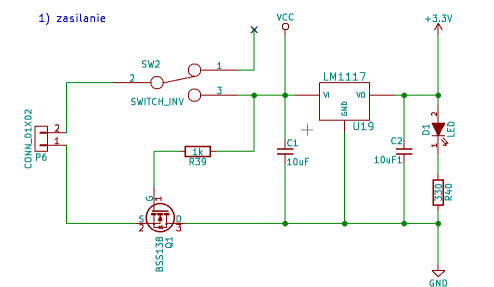
\includegraphics[scale=0.8]{zasilanie.png}
\caption{Zasilanie}
\vspace*{1cm}
\noindent \rule{\linewidth}{0.4mm}
\end{center}

%\begin{figure}[!ht]
%\centring
%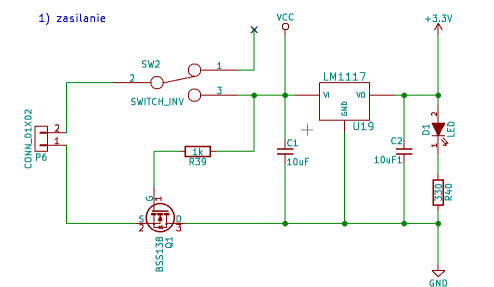
\includegraphics[scale=0.8]{zasilanie.png}
%\caption{Zasilanie}
%\label{CO TU WSTAWIC}
%\end{figure}

\subsubsection{Mikrokontroler}

Wybrano mikrokontroler STM32F051R8T6
\newline Specyfikacja:
\begin{itemize}
\item Typ układu scalonego: Mikrokontroler ARM
\item Pojemność pamięci Flash: 64kB
\item Częstotliwość taktowania: 48MHz
\item Montaż: SMD
\item Liczba wejść/wyjść: 55
\item Pojemność pamięci SRAM: 8kB
\item Obudowa: LQFP64
\item Napięcie zasilania: 2V - 3.6V DC
\item Rodzaj architektury: Cortex M0
\item Liczba timerów 16-bitowych: 7
\item Liczba timerów 32-bitowych: 1
\item Interfejs: I2C x2, SPI, UART x2
\item Masa: 2.12g
\end{itemize}

Początkowo mieliśmy użyć mikrokontrolera STM32F051C8T6, różni się tylko ilością dostępnych wejść i wyjść (tj. 39). Trafne było użycie powyższego mikrokontrolera ze względu na wygodniejszą możliwość konfiguracji peryferii.	 

\begin{center}
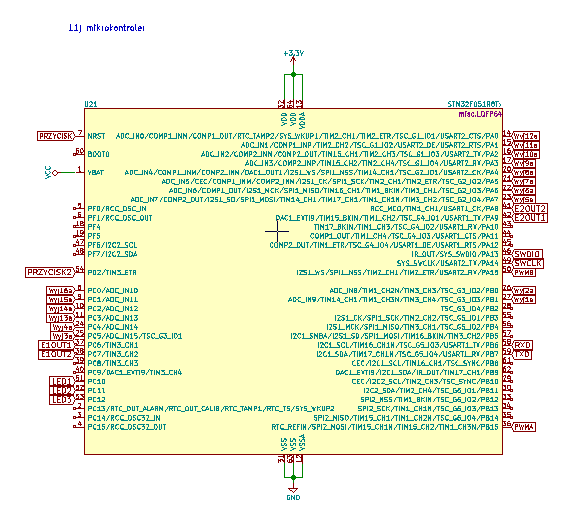
\includegraphics[scale=0.7]{mikroklocek1.png}
\caption{Mikrokontroler}
\vspace*{1cm}
\noindent \rule{\linewidth}{0.4mm}
\end{center}

\begin{center}
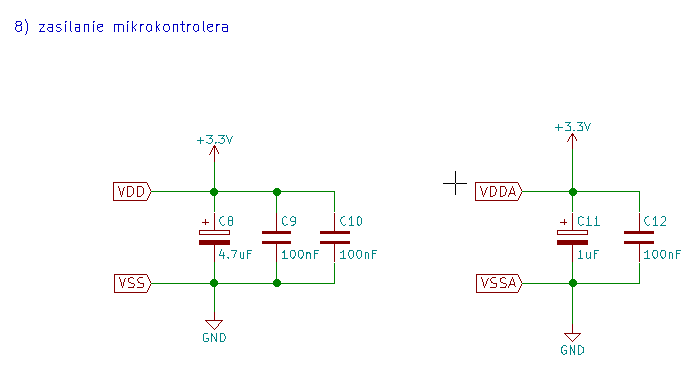
\includegraphics[scale=0.6]{zasilaniemikroklocka.png}
\caption{Zasilanie mikrokontrolera}
\vspace*{1cm}
\noindent \rule{\linewidth}{0.4mm}
\end{center}

\subsubsection{Czujniki}

Wybrano czujniki odbiciowe KTIR0711S
\newline Specyfikajca:
\begin{itemize}
\item Maksymalne napięcie diody IR: 5 V
\item Maksymalny prąd diody IR: 50 mA
\item Maksymalne napięcie kolektor-emiter: 30 V
\item Maksymalny prąd kolektora: 20 mA
\item Obudowa lutowana powierzchniowo (SMD)
\end{itemize}

\begin{center}
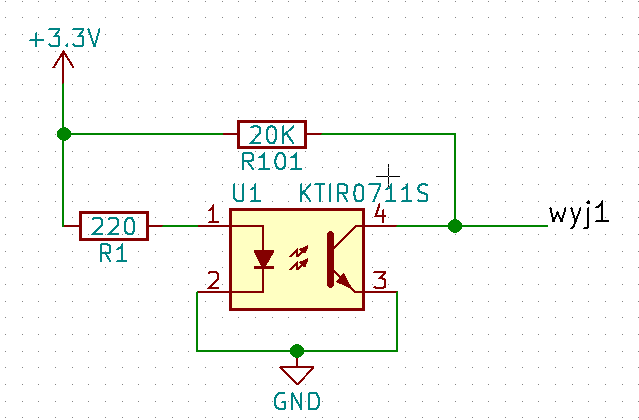
\includegraphics[scale=0.5]{KTIR.png}
\caption{Czujnik odbiciowy}
\vspace*{1cm}
\noindent \rule{\linewidth}{0.4mm}
\end{center}

\subsubsection{Sterowanie silnikami}

Wybrano dwukanałowy sterownik silników TB6612FNG
\newline Specyfikacja:
\begin{itemize}
\item Maksymalne napięcie zasilania silników: 4,5 - 15 V
\item Prąd ciągły 1,2 A
\item Prąd chwilowy: 3,2 A 
\item Tryb niskiego poboru prądu (Standby)
\item Możliwość zmiany kierunku obrotów silnika
\item Możliwość szybkiego zatrzymania silnika
\item Obudowa: SMD SSOP24
\item Kanały sterownika można połączyć aby otrzymać większą wydajność prądową
\end{itemize}

\begin{center}
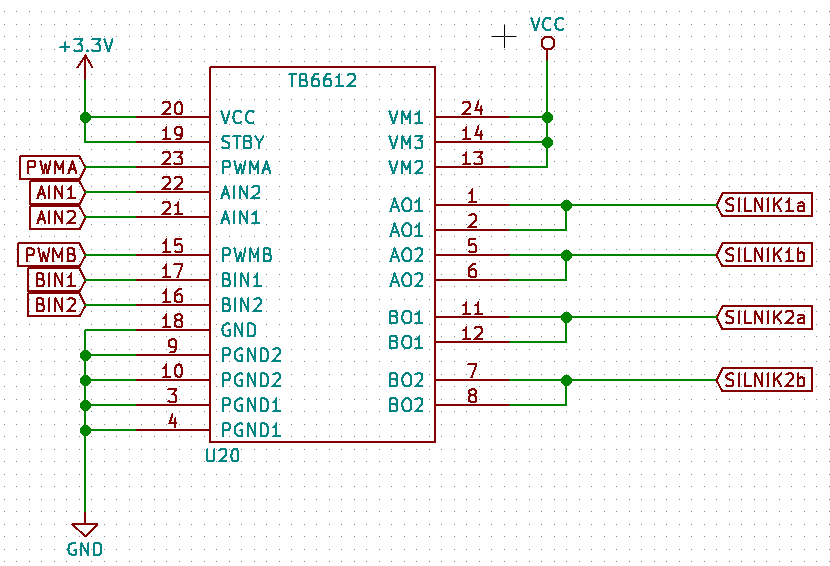
\includegraphics[scale=0.5]{tbek.png}
\caption{Mostek H}
\vspace*{1cm}
\noindent \rule{\linewidth}{0.4mm}
\end{center}

\begin{center}
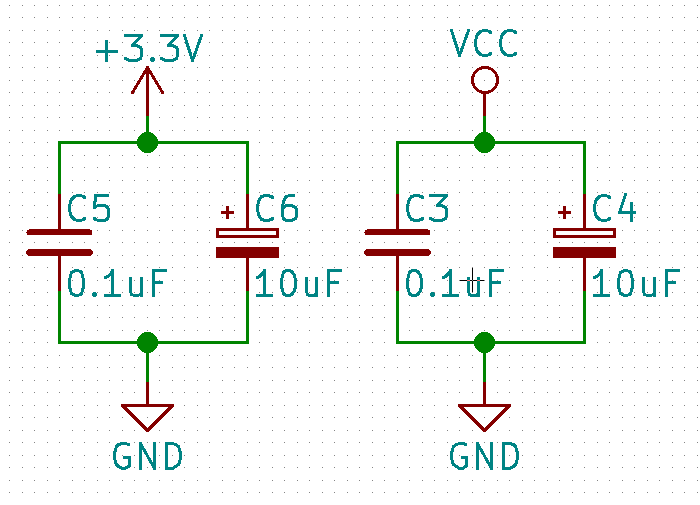
\includegraphics[scale=0.3]{zasilanietbka.png}
\caption{Zasilanie Mostka H}
\vspace*{1cm}
\noindent \rule{\linewidth}{0.4mm}
\end{center}

\subsubsection{Interfejs komunikacyjny}
%Jak można się komunikować z robotem --- przyciski, programator, bluetooth itp. oraz jak robot może się komunikować z nami --- diody led, buzzer (brzęczyk piezoelektryczny), moduł radiowy, bluetooth itp. Dlaczego tak i dlaczego nie włożyliśmy tam tego bluetootha? Schematy.

Z robotem komunikowaliśmy się za pomocą programatora z płytki Nucleo lub Discovery. Robot posiada trzy diody, z czego wykorzystaliśmy tylko dwie. Pierwsza dioda świecąc wskazywała na płynący prąd w obwodzie. Druga świeciła się po poprawnym wgraniu kodu ( ostatnia linija w kodzie zaświecała diodą ). Natomiast robot posiada moduł bluetooth lecz przez brak czasu zrezygnowaliśmy z programowania tego modułu zajmując się kalibracją robota.

\subsection{Program} 

Program był pisany w języku C, z wykorzystaniem biblioteki HAL. Korzystano z darmowego środowiska programistycznego dla mikrokontrolerów STM32. Do wygnerowania konfiguracji peryferiów użyto darmowego programu STM32CubeMX. System Workbench for STM32 to darmowe środowisko programistyczne w opraciu o Elipse. Pozwala to na programowanie jak i również debugowanie danych urządzeń. Bezcenne okazało się STMStudio do wizualizowania pracy czujników odbiciowych oraz STM32 ST-LINK Utility jako alternatywa do programowania i łączenia się z mikrokontrolerem.

\subsubsection{Konfiguracja peryferii}

Do wykrycia czarnej linii użyto ADC korzystające z DMA (Direct Memory Access, DMA (z ang. bezpośredni dostęp do pamięci)). Do regulacji obrotów zostało oparne na generacji sygnału PWM przez timer o częstotliwości taktowania 1000Hz. 
\newline Konifguracja timerów
\newline Dane:
\begin{itemize}
\item Prescaler (16-bitowy) = 47
\item Counter Mode = up
\item Counter Period = 999
\item Internal Clock Division = no division 
\end{itemize}
Pętla algorytmu sterownia robotem jest wykonywana w przerwaniu timera z częstotliwościa 100Hz.

\subsubsection{Algorytm sterowania}
%Opisujemy algorytm sterowania zastosowany w robocie. Można pokusić się o diagram czynności. Żadnego wklejania kodu na milion stron.

Do sterowania zastosowaliśmy algorytm PD (proporcjonalo-różniczkujący). Nie stosowaliśmy członu całkującego ponieważ komplikuje on układ i nie wnosi poprawy w sterowaniu. Regulator PD jest wykonywany w przerwaniu timera z częstotliwością 100Hz. Człon proporcjonalny jest odpowiedzialny za natychmiastową reakcję przy zakłóceniu jakim jest zmiana pozycje względem linii. Człon różniczkujący tłumi oscylacje robota.
\\
\newline Zasada działania:
\begin{description}
\item[1] \hfill \\
 Na początku pobierany jest odczyt z czujników i przetwożenie ich wartości w trybie DMA
\item[2] \hfill \\
Następnie na podstawie przypisanej wagi każdemu z czujników obliczany jest uchyb regulacji, od którego zależy prędkość silników
\item[3] \hfill \\
W kolejnym etapie podawana są nowe prędkości na każdy silnik 
\item[4] \hfill \\
Proces powtarza się tak z częstotliwościa 100Hz
\end{description}
Przy zerowym blędzie oba silniki mają taką samą ustaloną prędkość. W zależności od błędu jeden z silników będzie przyśpieszał a drugi zwalniał. Przy bardzo ostrym zakręci jeden z silnikó dostanie większą moc a drugi będzie się kręcił w przeciwną stronę. Ważnym elementem algorytmu jest zapamiętywanie błędu i ciągła ich aktualizacja. Wypadnięcie z trasy skutkować będzie zwiększonym uchybem. Wartości czujników są przypisane liniowo, natomiast skajne czujniki otrzymały większe wartości. 

\section{Podsumowanie}
W dokumencie opisano proces budowy robota klasy Line-Follower. Prace nad nim trwały nie całe 8 tygodni. Cel został osiągnięty, robot pojechał na zawodach Robotic Arena 2016. Dzień przed zawodami robot ostro bronił się przed wgraniem czegokolwiek, np. zaświecenie diodą. Podczas zawodów nie sprawiał żadnych problemów, program z poprawkami był wgrywany wielokrotnie. Przyczyny odmowy wgrania programu dzień przed zawodami są nieznane do dziś dzień. Natomiast godzinę przed rozpoczęciem naszej konkurencji spalił się stabilizator a później tranzystor. ( Na szczęście w moim zespole był szaman lutowania, 10 minut później robot ozdrowiał ). Mjølner poradził sobie bardzo dobrze, w klasie Line-Follower Light uzyskał 9 miejsce. Podsumowując, robot okazał się dobrą kontrukcja i po dwóch miesiącach starań pojechał na zawodach. Jest jednak jeszcze wiele do zrobienia.
\\
\newline Cele na przyszłość:
\begin{itemize}
\item oprogramowanie modulu bluetooth
\item oprogramowanie enkoderów
\item ulepszenia algorytmu (człon całkujący)
\item zapis programu strukturalnie, z podziałem na funkcje
\item przetestowanie silników z przekładnią 10:1
\end{itemize}

%Tutaj można też wkleić więcej zdjęć robota z różnych ujęć.

\section{Materiały źródłowe}
Tutaj możemy napisać skąd czerpaliśmy wiedzę - np. z warsztatów, z Forbota, z płyt chodnikowych pod domem.
Warto także wskazać na czym oparło się swoją pracę, np. tak \cite{buka}.

\bibliographystyle{plunsrt}
\bibliography{mybib}
\clearpage



\end{document}